\section{Data Collection}%Methodology to collect VirusTotal data}

%\subsection{The large data set}

%How the data set is built?

%What information we can get? Basically, we need to explain the data format. 

%Basic properties of the data set

%a. How many submissions every data?

%b. Submission type distribution

%c. The number of submissions for the same file

%d. Engines used to scan a submission 

%Advantage: 

%Across categorization, such as file types 

%Covering a longer time.

In this section, we introduce how we collect data. 

\subsection{Methodology}

First, we introduce our data source, VirusTotal, and how we make use of their APIs. VirusTotal offers a lot of APIs for researchers. Their private APIs could return the detailed detection results of vendors. We applied for a private API key for our data collection. We mainly use two APIs for collecting data: \texttt{report} and \texttt{rescan}. \texttt{report} takes a hash value of a sample as input, and returns a detailed report of the sample if the sample exists in the library of VirusTotal. The report contains the detection results of the sample from all the vendors that VirusTotal could provide. \texttt{rescan} also takes a hash value as input. This API sets VirusTotal to rescan the specified sample. This could make VirusTotal to update the detection results of samples.

Then we introduce how to collect the data set. 
First, at day 0, we obtained about 14,423 new Portable Executable (PE, the executable file format on Windows) files from an anti-virus vendor. 
We then submitted the 14423 files to VirusTotal at the same day, and got the detection results from VirusTotal. 
None of these files were submitted to VirusTotal prior to day 0.
For each day later on, we first call \texttt{rescan} on the 14423 files respectively. Then, we wait 2 hours for VirusTotal updating the detection results. 
After 2 hours, we call \texttt{report} on each files to get the updated detection results. 
We keep collecting data for 75 days. 

\subsection{What information can we get from VirusTotal?}% I mean the data format. 

The API \texttt{report} returns a lot of information of the sample, including but not limited to hashcodes (MD5, SHA1, etc.) of the sample, scan date, and detailed scan results of many vendors. For each vendor in the detailed scan results, there are 4 fields: \texttt{detected}, \texttt{version}, \texttt{result}, and \texttt{update}. \vt\ does not provide detailed documentation of the fields, but it is easy to infer from the results and other documents (such as https://www.virustotal.com/en/faq/). \texttt{detected} tells if the sample is detected as malicious by this vendor. \texttt{version} tells the version used in the scan. \texttt{result} is how the vendor classifies the sample. \texttt{update} is the date of the vendor providing the anti-virus tool.

\subsection{Basic properties of the data set}

Now we take a look at the data set. First, there are 7197 malicious files and 7226 benign files according to the results from first scan. We say ``malicious'' as long as there is one vendor reporting malicious. This indicates that our dataset is balanced.

Then we check the completeness of the dataset by observing two distributions. 
Our dataset could be regarded as a set of tuples $(f, v, t)$ that sample $f$ is scanned at time $t$ by vendor $v$. Ideally, there should be one tuple for all $f, v, $ and $t$ in all 14423 files, more than 70 vendors and 75 days. 
However, not all valid tuples exist in the downloaded information. Some tuples may miss because of VirusTotal or our crawling configuration. So we calculated two distributions of the data set to check the completeness.
First, Figure~\ref{fig:dataset_submission_vendor_distri} shows the distribution of how many vendors have scanned a sample in a detection result. A point $(x, y)$ on the curve represents that there are $y$ detection results with $x$ vendors scanned. From the chart, we can know that most of the detection results are detected by more than 65 vendors. 
In addition, Figure~\ref{fig:dataset_no_vendors_scanned_moste_files_in_x_days} shows  how many vendors scan most of the files in how many days. More specifically, $(x, y)$ in the chart represents there are $y$ vendors that scans more than 90\% of the total files in $x$ days. The figure indicates that most of the vendors 
From the two figures, we could conclude that the dataset is mostly complete.

\begin{figure}
\centering
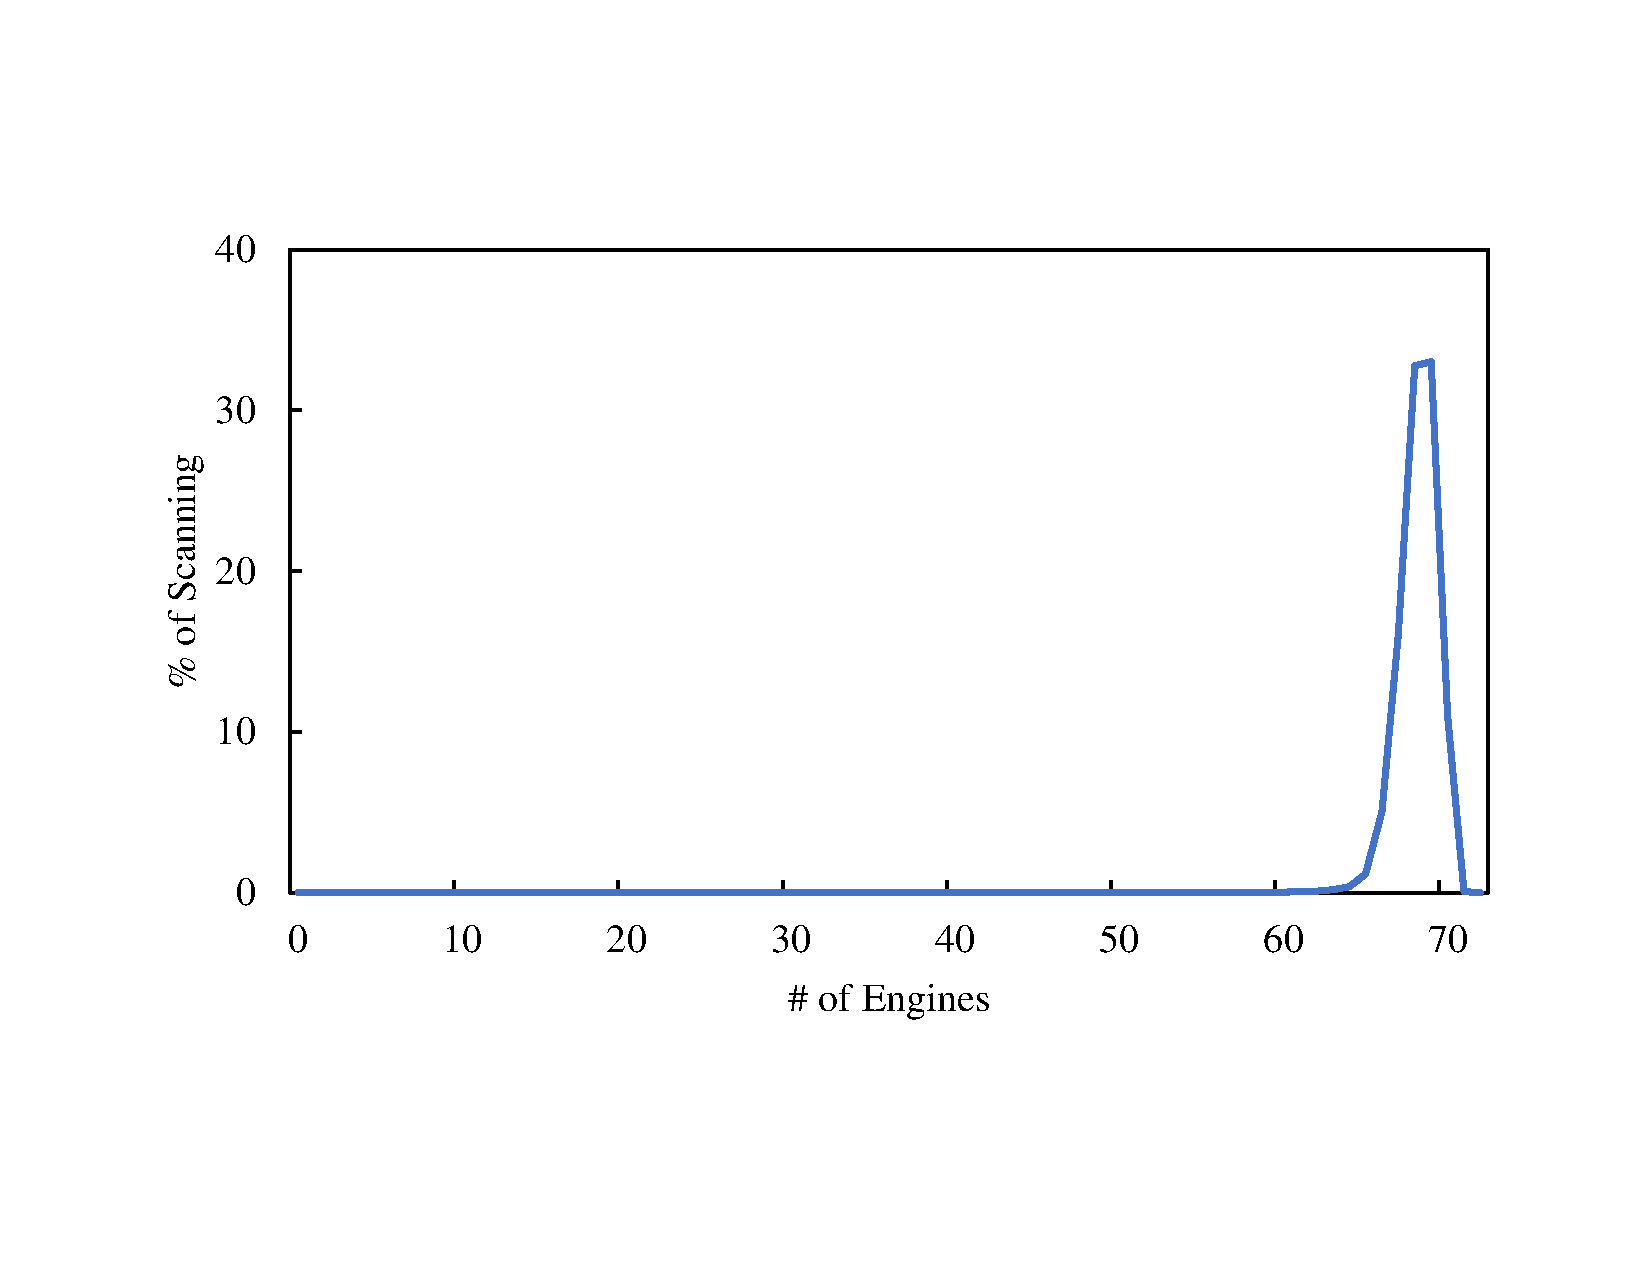
\includegraphics[width=0.7\linewidth]{figure/vendor_submission_distribution}
\caption{Distribution of detection results vs. vendors}
\label{fig:dataset_submission_vendor_distri}
\end{figure}

\begin{figure}
\centering
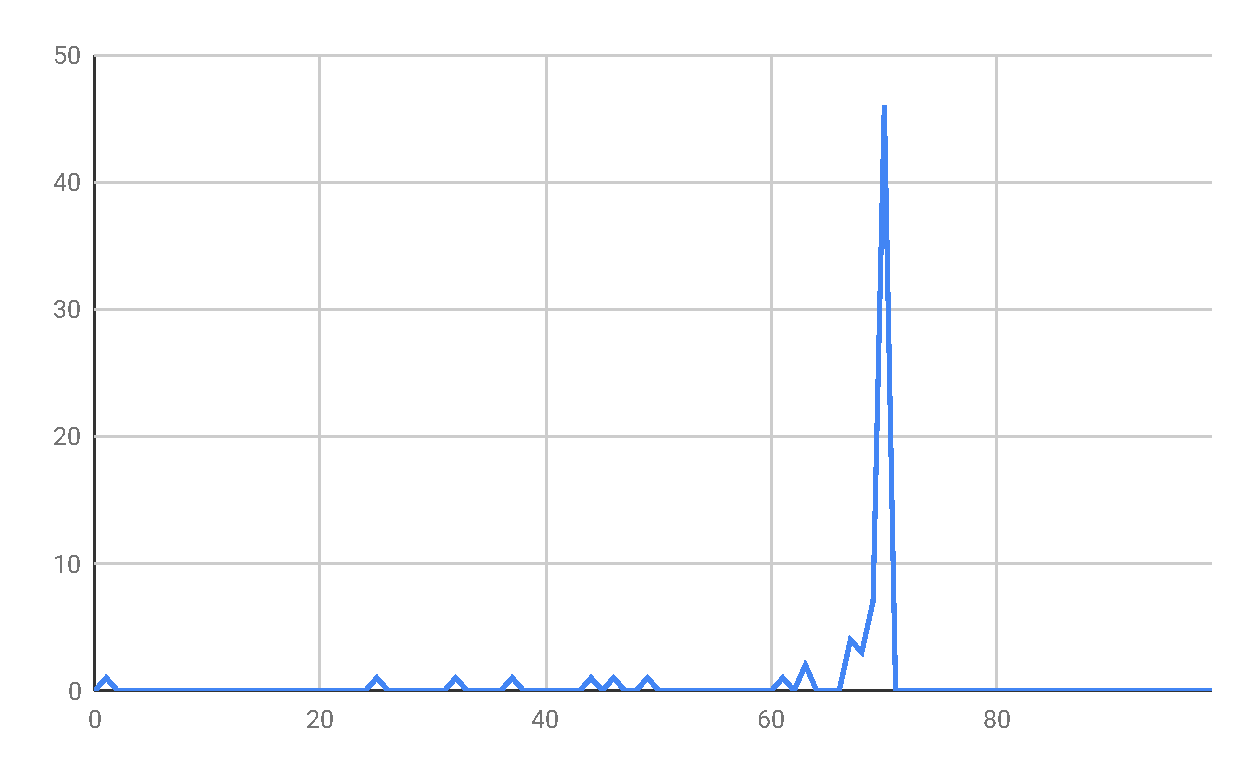
\includegraphics[width=0.7\linewidth]{figure/dataset_no_vendors_scanned_moste_files_in_x_days}
\caption{the number of vendors that scanned more than 12980 (>90\%) files in $x$ days}
\label{fig:dataset_no_vendors_scanned_moste_files_in_x_days}
\end{figure}


\subsection{How VirusTotal update engines?}
As we mentioned above, we use \texttt{rescan} and \texttt{report} to get the latest detection results from VirusTotal for each day. Actually, how VirtusTotal update the antivirus engines? With our data set for 75 days, we first check whether antivirus bases and versions update over time. We find that more than 78\% of the detection results updates consistently with time went on. So we can get new detection results from VirusTotal when we \texttt{rescan} samples and \texttt{report} detction results 2 hours later.


\begin{figure}
\centering
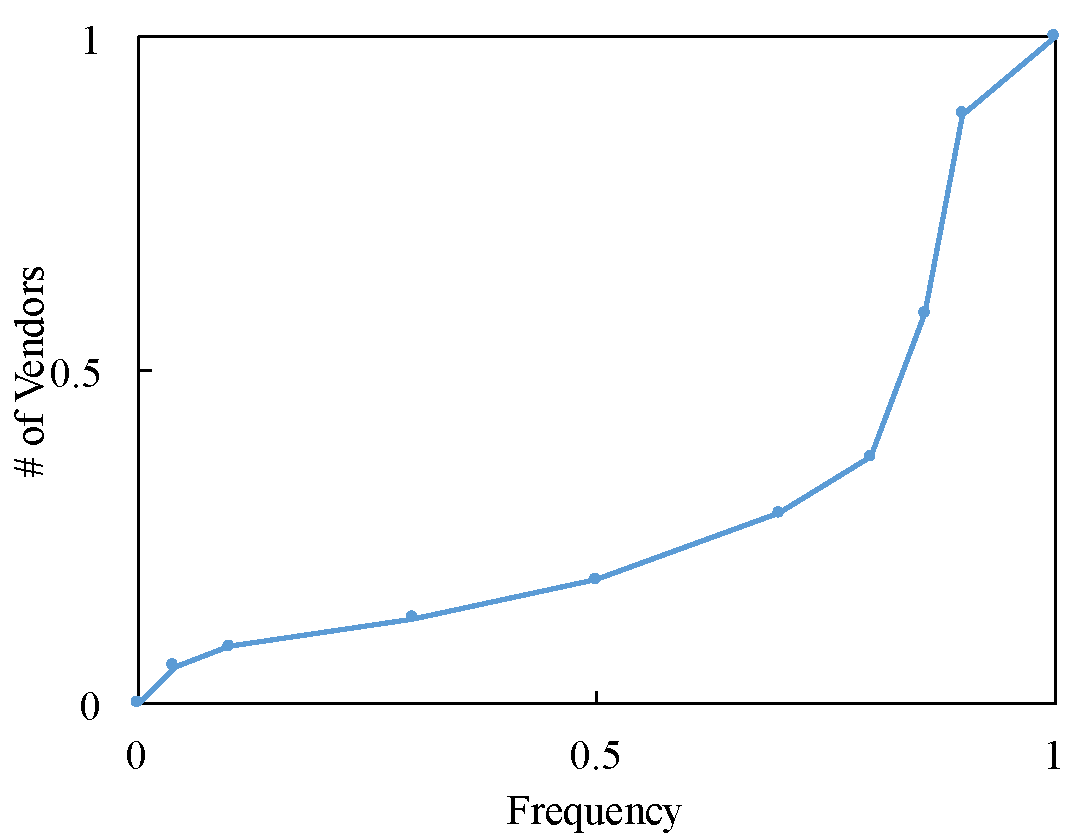
\includegraphics[width=0.7\linewidth]{figure/frequency}
\caption{Distribution of update frequency over vendors.}
\label{fig:frequency}
\end{figure}

Figure \ref{fig:requency} presents the distribution of updating frequency for vendors. Overall, more than 44 vendors(total 70) update their detction results with at least 1 day. Only 6 vendors' updating frequency are less than 0.05, and 4 of them seems not change their antivirus engines during these 75 days. Averagely, about 56 vendors will be updated with at least 2 days. 

%c. How VirusTotal update engines? Scanning time vs. update vs. version 
%TODO: need more data
\subsection{Caveats}

Discuss errors during our data collection. 
